\documentclass[12pt,a4paper]{article}


% Packages
%======================================
% Page Geometry
\usepackage[DIV=14,BCOR=2mm,headinclude=true,footinclude=false]{typearea}
%======================================
% Document spacing
% Line spacing
\usepackage{setspace}
\setstretch{1.2}
% Paragraph spacing
\usepackage[skip=2.5pt, indent=12pt]{parskip}
%======================================
% Headers and footnotes
\usepackage{fancyhdr}
%======================================
% Math packages
\usepackage{tikz}
\usepackage{physics}
\usepackage{tikz-cd}
\usepackage{mathtools}
\usepackage{amsmath,amssymb}
% Quotient space
\newcommand{\bigslant}[2]{{\raisebox{.2em}{$#1$}\left/\raisebox{-.2em}{$#2$}\right.}}
%======================================
% Theorem environments
\usepackage{amsthm}
\newtheorem{theorem}{Theorem}[section]
\newtheorem{lemma}[theorem]{Lemma}
\newtheorem{corollary}{Corollary}[theorem]
% Definition style
\theoremstyle{definition}
\newtheorem{definition}{Definition}[section]
% Remark style
\theoremstyle{remark}
\newtheorem{remark}{\textit{Remark}}[section]
% Example style
\theoremstyle{definition}
\newtheorem{example}{Example}[section]
%======================================
% German ß ä ö ü
\usepackage[T1]{fontenc}
\usepackage[main=english,german]{babel}
%======================================
% Color
\usepackage{xcolor}
\definecolor{TUColor}{cmyk}{0, 1.0, 0.99, 0.40} % TU Dark Red
\definecolor{CitationColor}{cmyk}{0.9, 0.6, 0.0, 0.6} % Dark Blue
\definecolor{RichBlack}{cmyk}{0.75, 0.68, 0.67, 0.9}
%======================================
% Hyper links and references
\usepackage{hyperref}
\hypersetup{
    colorlinks,
    urlcolor={CitationColor},
    citecolor={CitationColor},
    linkcolor={RichBlack}
}
%======================================
% Citations
\usepackage[nobreak]{cite}
%======================================
% Images
\usepackage{float}
\usepackage{graphicx}
\graphicspath{{./images/}}
% Captions
\usepackage{subcaption}
\renewcommand\thesubfigure{\roman{subfigure}}
%======================================
% For Title page
\usepackage{tabularx,booktabs}
%======================================
% Fancy boxes
\usepackage[most]{tcolorbox}
\tcbuselibrary{skins,breakable}
\newtcolorbox{mybox}[2][]{breakable, sharp corners, boxrule=0mm, leftrule=2mm, boxsep=0mm, arc=0mm, outer arc=0mm, opacityframe=0}
%======================================


\begin{document}
%===========================================================
% General settings
% Font color
\color{RichBlack}
% Redefine header "fancy" style
\fancypagestyle{fancy}{
    \fancyhead{}
    \fancyfoot{}
    \fancyhead[LE,RO]{\footnotesize\itshape\nouppercase{\rightmark}}
    \fancyhead[LO,RE]{\footnotesize\itshape\nouppercase{\leftmark}}
    \fancyfoot[C]{\footnotesize\itshape\nouppercase\thepage}
    \renewcommand{\headrulewidth}{0.4pt}
    \renewcommand{\footrulewidth}{0.0pt}
}
\fancypagestyle{tocstyle}{
  \fancyhead{}
  \fancyfoot{}
  \renewcommand{\headrulewidth}{0.4pt}
  \renewcommand{\footrulewidth}{0.0pt}
}
%===========================================================


% Title page
%===========================================================
\begin{titlepage}
% Defines a new command for horizontal lines, change thickness here
\newcommand{\HRule}{\rule{\linewidth}{0.5mm}}
\begin{center}


\includegraphics[width=0.15\textwidth]{TU-Berlin-Logo.png}\\[1cm]
\begin{otherlanguage}{german}
\textsc{\LARGE Technische Universit"at Berlin}\\[1.5cm]
\textsc{\large Fakult\"at 2}\\[0.5cm]
\textsc{\large Institut f\"ur Mathematik}\\[0.5cm]
\end{otherlanguage}

% Title
\setlength{\aboverulesep}{10pt}
\setlength{\belowrulesep}{13pt}
\begin{tabularx}{\textwidth}{ >{\centering\arraybackslash}X}
\midrule[0.5mm]
\huge\bfseries Circular cross sections of quadrics\\
\midrule[0.5mm]
\end{tabularx}

% Author and supervisor
\begin{minipage}{0.4\textwidth}
    \begin{flushleft}
        \large
        \textit{\textcolor{TUColor}{Author}}\\
        Sara \textsc{Samy}
    \end{flushleft}
\end{minipage}
~
\begin{minipage}{0.4\textwidth}
    \begin{flushright}
        \large
        \textit{\textcolor{TUColor}{Supervisor}}\\
        Dr. Jan \textsc{Techer}
    \end{flushright}
\end{minipage}

% Position the date 3/4 down the remaining page
\vspace{260 pt}
{\large\today}
\end{center}
\end{titlepage}
%===========================================================


%===========================================================
% Set Abstract page style to "fancy"
\pagestyle{fancy}
\section*{Abstract} \label{sec:abstract}
\pagebreak
%===========================================================
% Set TOC page style to "tocstyle"
\pagestyle{tocstyle}
\renewcommand{\contentsname}{Contents}
\tableofcontents
\pagebreak
%===========================================================
\listoffigures
\pagebreak
%===========================================================
% Set all following pages style to "fancy"
\pagestyle{fancy}
\section{Introduction} \label{sec:introduction}
\pagebreak
%===========================================================
\section{Circular sections of quadrics}
As mentioned in the \hyperref[sec:introduction]{introduction}
\begin{align} \label{eq:Euler}
    e^{i \theta} = \cos(\theta)+i\sin(\theta)
\end{align}
The \hyperref[eq:Euler]{equation} as given is..
\pagebreak
%===========================================================
\section{Families of confocal quadrics}
\begin{definition}[Confocal quadrics]
\label{def:confocal-quadrics}
Two quadrics are \textit{confocal}, sometimes also referred to as \textit{homofocal}, if they have common axes and intersect each plane of symmetry along confocal conics.
\end{definition}
A classical system of confocal quadrics in Euclidean space $\mathbb{R}^3$ is composed of three families of quadrics given by
\pagebreak
%===========================================================
\section{Lines of curvature on confocal quadrics}
\pagebreak
%===========================================================
\section{Diagonally related nets on surfaces}
We start by defining nets on surfaces. Mutually diagonal nets on surfaces were introduced in \cite{MutuallyDiagonalNets2019}.

\begin{definition}[Nets on surfaces]
\label{def:nets-on-surfaces}
A net $\mathcal{N}$ on a surface $\Sigma$ is a pair of one-parameter families of curves on $\Sigma$, such that for every point on $\Sigma$ there exists exactly one curve from each of the two families through that point.
\end{definition}

\begin{remark}[]
\label{rm:label}
Let $\mathcal{N} = \left( (\alpha_{s_{1}})_{s_{1} \in I_1}, (\beta_{s_{2}})_{s_{2} \in I_2} \right)$ be a net on a surface
$\Sigma$ and $P$ a point on the surface then there exists a unique pair $(s_{1}, s_{2}) \in I_{1}\times I_{2}$ such that
\[
    P = \alpha_{s_1} \cap \beta_{s_2}
\]
We call $(s_1, s_2)$ the \textit{coordinates of the point $P$ with respect to the net $\mathcal{N}$}. Note that these coordinates alone do not uniquely determine the points on the surface, especially that we don't assume that each two curves from different families of $\mathcal{N}$ intersect in one unique point. However, the net together with a specific parameterization of its curves uniquely determine the points of the surface.
\end{remark}

\begin{example}
\label{ex:nets-on-surfaces}
Let $\varphi : I_{1} \times I_{2} \subset \mathbb{R}^2 \to \mathbb{R}^3$ be a parameterization of a surface. Then its
coordinate lines, i.e. the curves
\begin{align*}
    \varphi_{u_0} : I_{2} \to \mathbb{R}^3 &\quad \quad \varphi_{u_0}(v) = \varphi(u_0, v), \text{ and} \\
    \varphi_{v_0} : I_{1} \to \mathbb{R}^3 &\quad \quad \varphi_{v_0}(u) = \varphi(u, v_0)
\end{align*}
defined for each fixed $u_{0} \in I_1, v_{0} \in I_2$ constitute a net on the surface $\varphi\left( I_1 \times I_{2}
\right) \subset \mathbb{R}^3$.
\end{example}

\begin{figure}[!tbp]
  \begin{subfigure}[b]{0.5\textwidth}
    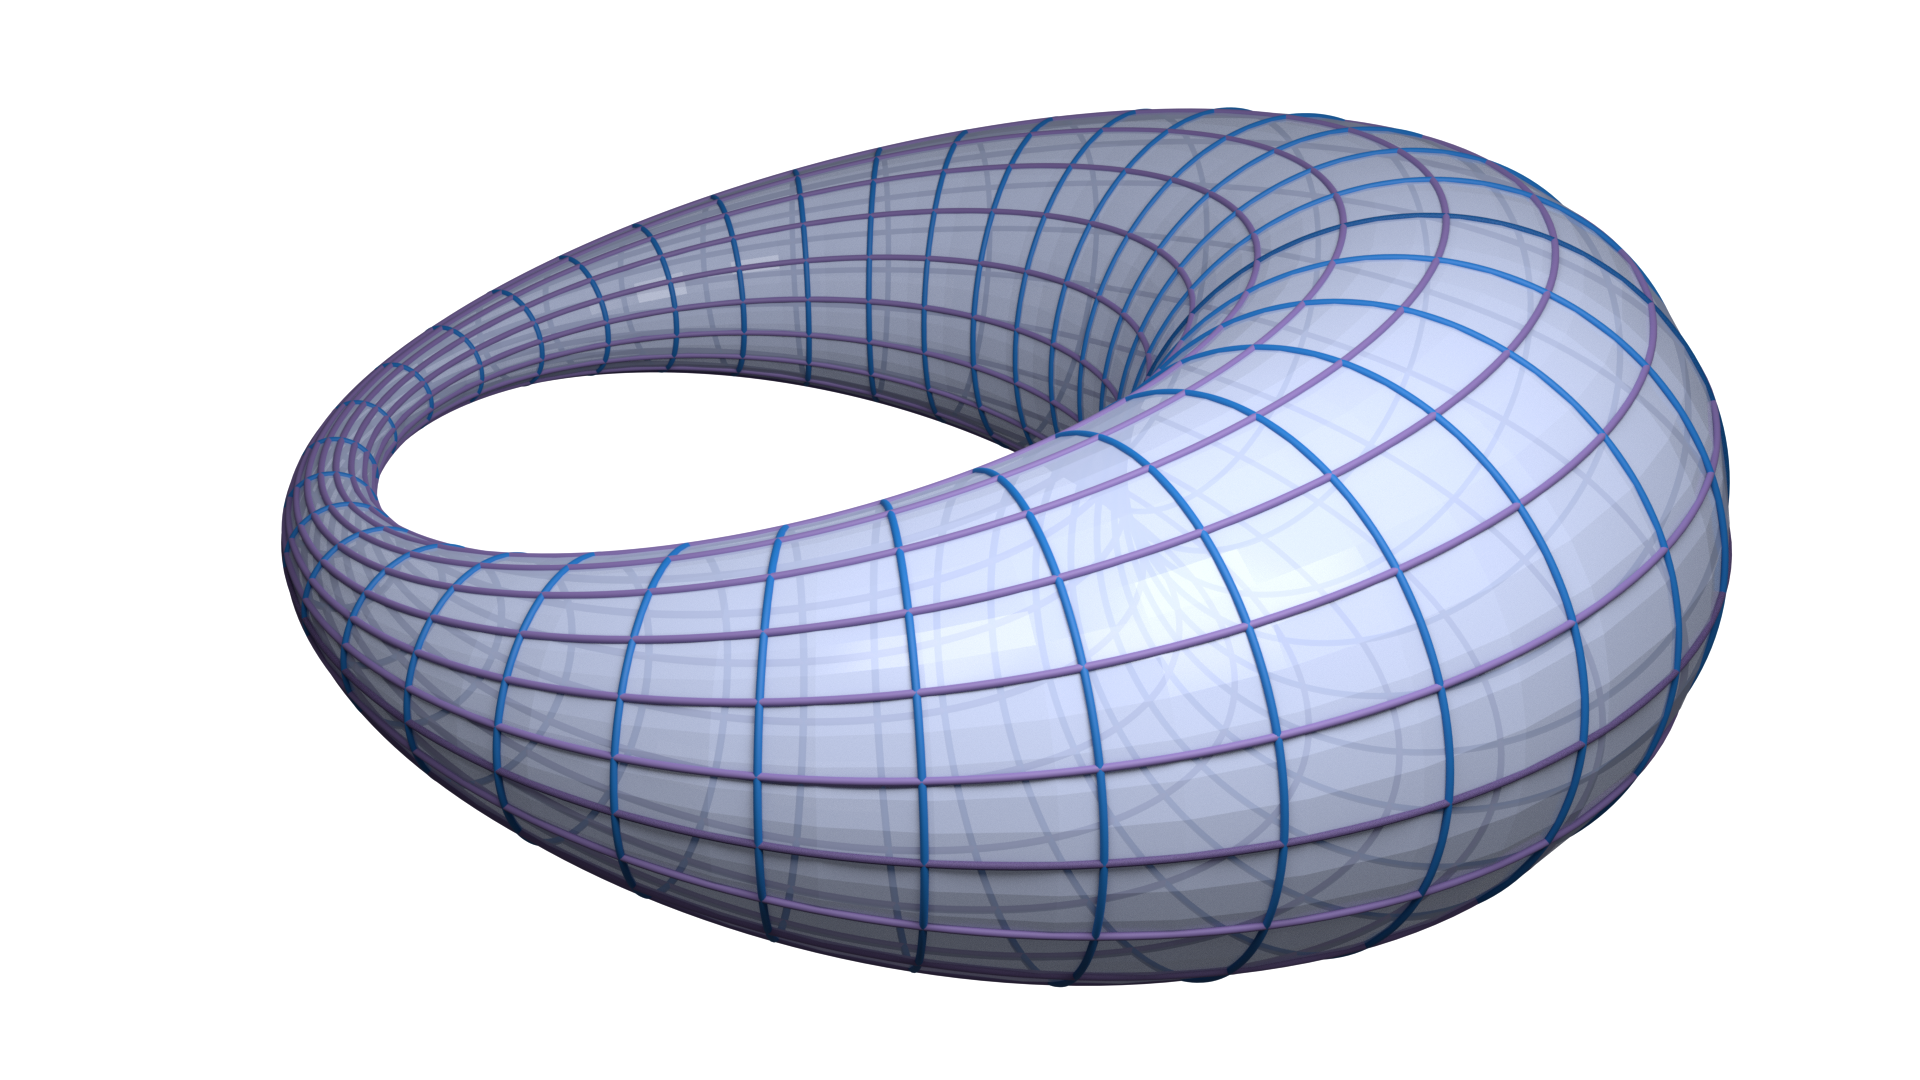
\includegraphics[width=\textwidth]{Dupin-net.png}
    \caption{ellipto-hyperbolic}
    \label{fig:ellipto-hyperbolic-cyclides}
  \end{subfigure}
  \hfill
  \begin{subfigure}[b]{0.5\textwidth}
    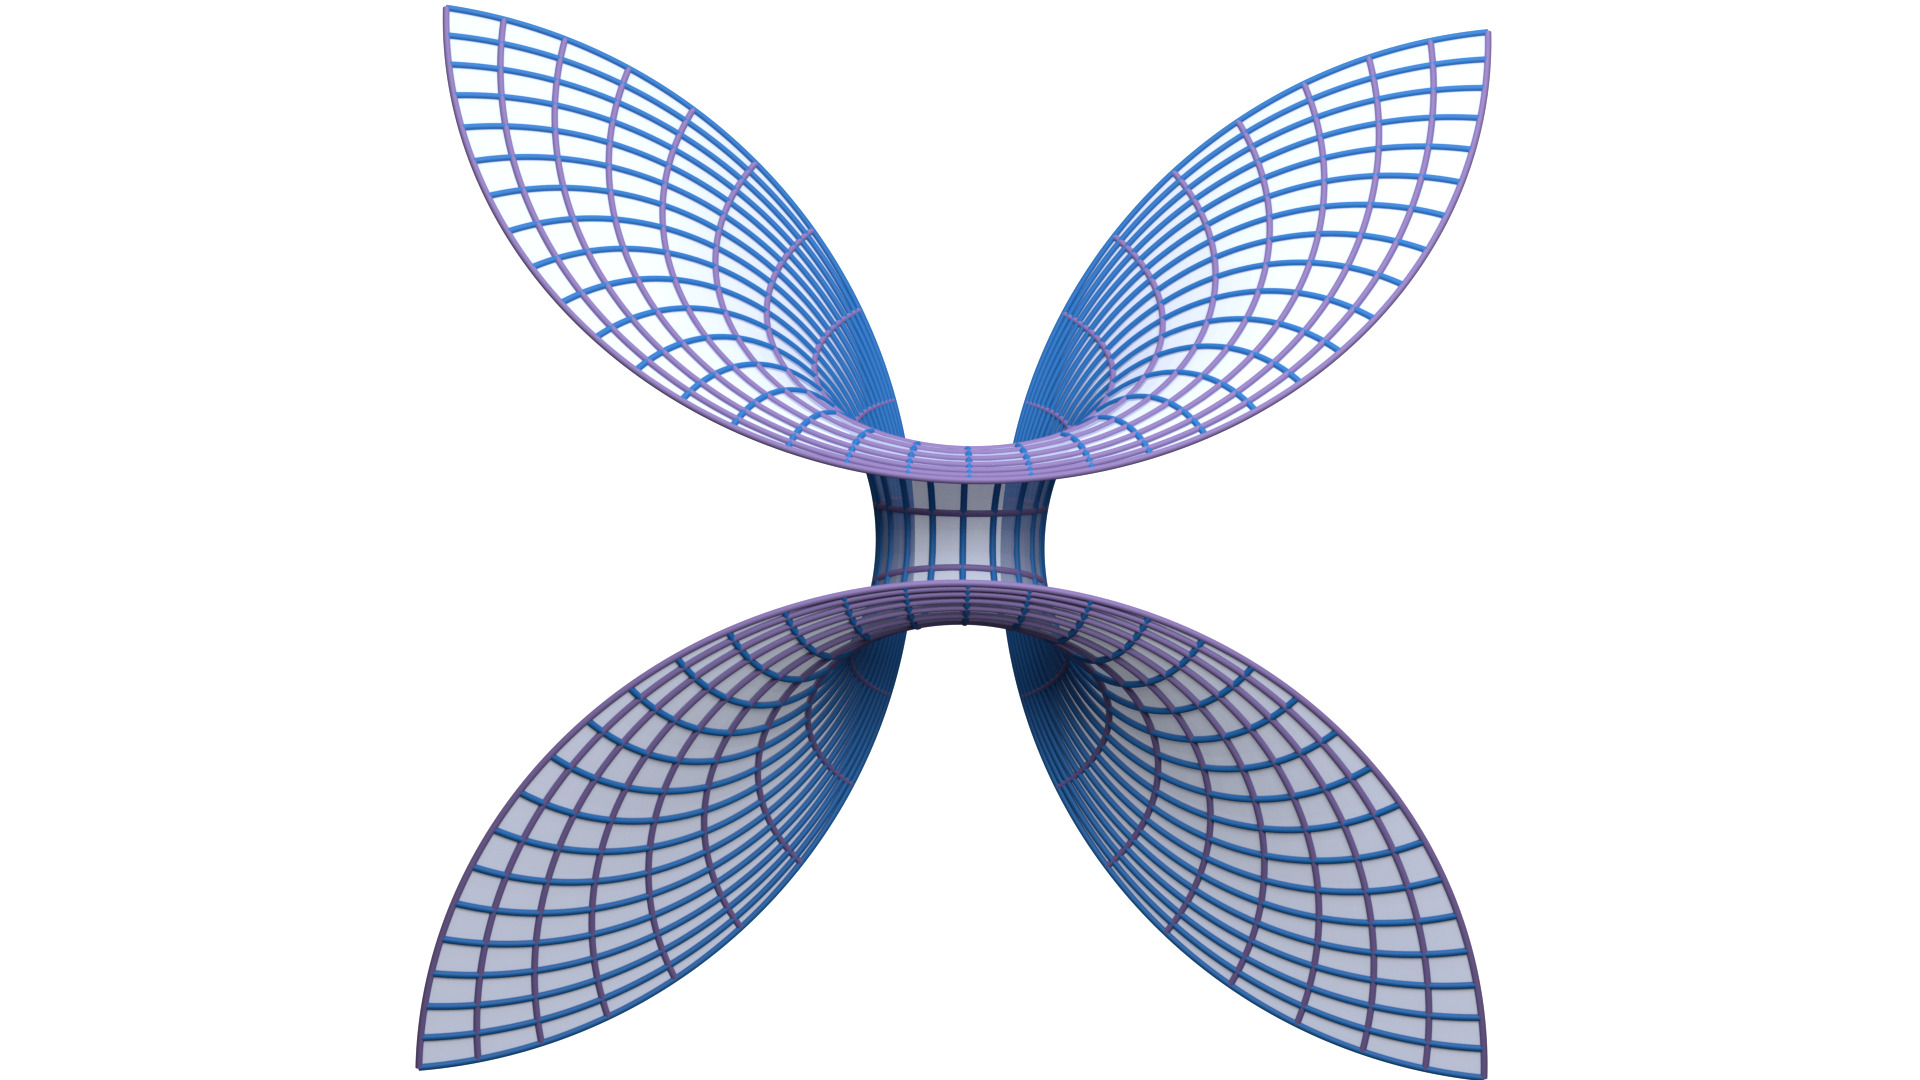
\includegraphics[width=\textwidth]{Dupin-net-2.png}
    \caption{parabolic}
    \label{fig:parabolic-cyclides}
  \end{subfigure}
  \caption{Dupin Cyclides}
\end{figure}

An interesting relation to nets on surfaces is the notion of a \textit{map} \cite{} which is an embedding of a connected
graph or multigraph $X$ into a surface $\Sigma$, such that all of the components of $\Sigma \setminus X$, called
the faces of the map, are homeomorphic to unit disks. The face-size $m$ and the vertex-degree $k$ give its type $\{m, k\}$.

\begin{definition}[Diagonally related nets on surfaces]
\label{def:diag-nets-on-surfaces}
Let $\mathcal{N}_{1}$ and $\mathcal{N}_{2}$ be two nets on a surface $\Sigma$. Then $\mathcal{N}_{2}$ is called diagonal
to $\mathcal{N}_{1}$ if the following condition is satisfied whenever any four curves of $\mathcal{N}_{1}$ form a
(combinatorial) quadrilateral:\\
\begin{mybox}{}
If one pair of opposite vertices is connected by a curve from $\mathcal{N}_{2}$, then the other pair of opposite vertices is connected by a curve from $\mathcal{N}_{1}$.
\end{mybox}
\end{definition}

\begin{figure}[h]
    \centering
    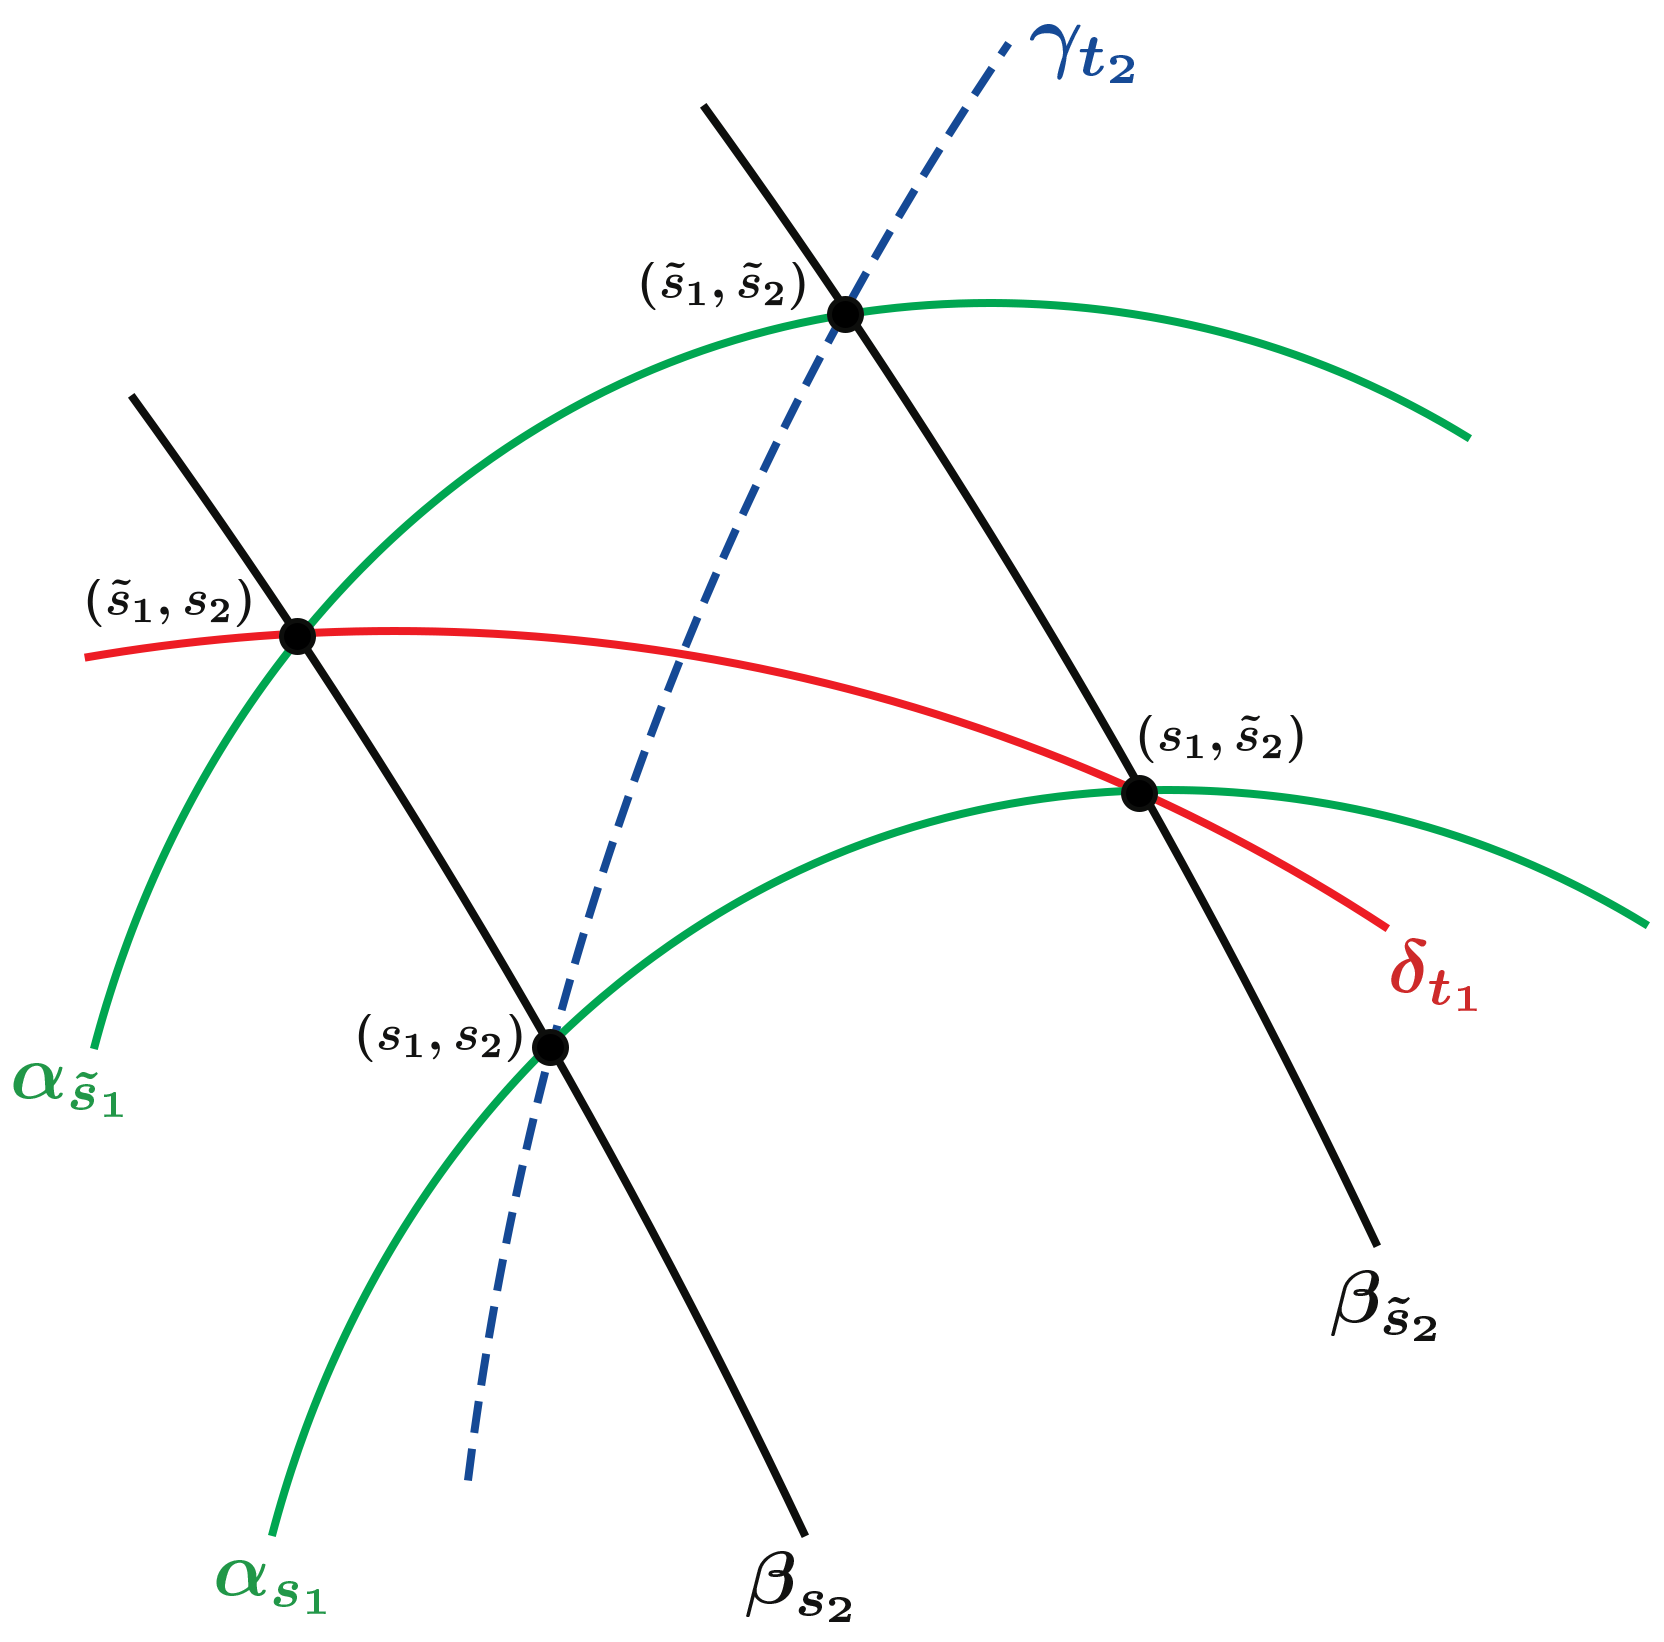
\includegraphics[width=0.5\textwidth]{diagonally_related_diagram.png}
    \caption{An illustration of the diagonal relation between two nets.}
    \label{fig:diagonally-related-nets}
\end{figure}

\begin{theorem}[]
\label{thm:symmetric-definition-diagonal-nets}
Let $\mathcal{N}_1$ and $\mathcal{N}_2$ be two nets on a surface $\Sigma$. Then $\mathcal{N}_1$ is diagonally related to
$\mathcal{N}_2$ if and only if $\mathcal{N}_2$ is diagonally related to $\mathcal{N}_1$.
\end{theorem}

\begin{proof}
    The proof
\end{proof}

\subsection{Diagonally related parameterizations}
\pagebreak
%===========================================================
\section{Diagonally related parameterization of hyperboloids}
\subsection{Diagonally related parameterization of one-sheeted hyperboloid}
\subsection{Diagonally related parameterization of two-sheeted hyperboloid}
\pagebreak
%===========================================================
\section{Isometric deformation of circular cross sections of hyperboloids}
\section{Isometric deformation of one-sheeted hyperboloid}
\section{Isometric deformation of two-sheeted hyperboloid}
\begin{theorem}
\label{thm:affine-transformation-hyperboloid}

\end{theorem}
%===========================================================
\section{Further related work}
\subsection{Confocal paraboloids}
\pagebreak
%===========================================================
\appendix
\section{Curvature line parameterizations}
\pagebreak
%===========================================================
\section{Discrete confocal quadrics}
\pagebreak
%===========================================================


%===========================================================
% Set page style to "tocstyle"
\pagestyle{tocstyle}
\addcontentsline{toc}{section}{References}
\bibliographystyle{alpha}
\bibliography{refs}
%===========================================================


\end{document}
